\documentclass[12pt]{article}
\usepackage{fullpage}
\usepackage[utf8]{inputenc}
\usepackage{graphicx}
\usepackage[english]{babel}
\usepackage{float}
\usepackage{natbib}
\usepackage{authblk}
\usepackage{url}
\usepackage[section]{placeins}
\usepackage{wrapfig, framed}

\title{\textbf{Project 5 Report : Compare clustering methods}}
\author{Sajal Kumar}
\date{}

\begin{document}
\maketitle

\section*{Implementation details on parameters}

My implementation uses all 4 methods : Kmeans clustering, Agglomerative clustering at Scipy, Agglomerative clustering at Sklearn and DBSCAN on their default setting except the following general parameters that could be changed:

\begin{itemize}
\item \texttt{random\_state} : Random seed (set to 1 by default).
\item \texttt{n\_jobs} : Number of parallel threads allowed (set to 4 by default).
\item \texttt{dist\_metric} : To compute distance between two points (sample) (set to `euclidean' by default).
\item \texttt{n\_cluster} : Number of clusters (set to `auto' by default, estimated by the `Elbow' method).
\end{itemize}

My implementation allows changes to the following clustering algorithm specific parameters:

\begin{itemize}
\item Agglomerative Clustering (at Scipy)
\begin{itemize}
\item \texttt{method} denoted by \texttt{linkage\_method} (set to `ward' by default).
\end{itemize}
\item Agglomerative Clustering (at Sklearn)
\begin{itemize}
\item \texttt{linkage} denoted by \texttt{linkage\_method} (set to `ward' by default).
\end{itemize}
\item DBSCAN
\begin{itemize}
\item \texttt{eps} denoted by \texttt{eps\_dbscan} (set to `auto' by default, estimated by the nearest neighbor method).
\item \texttt{min\_samples} denoted by \texttt{min\_pts\_dbscan} (set to `auto' by default, estimated by the nearest neighbor method).
\end{itemize}
\end{itemize}

Apart from the above mentioned parameter some other clustering algorithm specific parameters were changed but were not provided to the user:

\begin{itemize}
\item Kmeans
\begin{itemize}
\item \texttt{max\_iter} was set to 100.
\end{itemize}
\item DBSCAN
\begin{itemize}
\item \texttt{algorithm} was set to `kd\_tree'.
\end{itemize}
\end{itemize}

The above represents the `standard' setting for all regression methods when no parameter is changed. 

\subsection*{The Elbow method for estimating n\_cluster}

The `Elbow' method has been implemented in a separate class called \texttt{ClustUtility}. There were slight modifications made to the method in order to effectively pick a good \texttt{n\_cluster} automatically.

A k\_max was setup to avoid going over all $n$ samples. It represents the maximum number of k the `Elbow' method would check, it was computed as : 
\begin{equation}
k\_max = round(\frac{n}{0.05 \cdot n})
\end{equation}

The idea was to push the requirement of min cluster size $=$ 5\% of data.

Next, the distortion (mse) was computed for each k $\in [1, k\_max]$ :
\begin{equation}
mse = \frac{1}{k} \sum_{i}^{n} \left( x^{i} - \mu_{k} \right)^2
\end{equation}

where $\mu^{i}$ represents the centroid of cluster $k$. In this case, $mse$ is a better measure than $sse$ as we want to compute the average pollution in each cluster as the $k$ increases.

Next to determine a good $k$, the following cost function was computed :

\begin{equation}
cost = mse + k \cdot || C ||_1
\end{equation}

where $|| C ||_1$ is the l1 norm of $C$, that is, $range(1, k+1)$ or the unique labels in $k$ clusters. This idea was borrowed from Lasso regression. It is known the the $mse$ will decrease with increase in $k$, however, $k \cdot || C ||_1$ will heavily penalize larger $k$, causing an increase in the overall $cost$ after certain $k$. The last $k$ that did not improve the $cost$, that is, the penalty term was heavier than $mse$ (or the $mse$ was not significant enough), was chosen as the appropriate $k$. It worked quite well in my humble opinion, atleast for Iris, it did pick 3 clusters which should be the optimal number. Figure~1 shows the $k$ picked up for Iris and Faulty Steel Plates dataset.

\begin{figure}
\begin{minipage}{\linewidth}
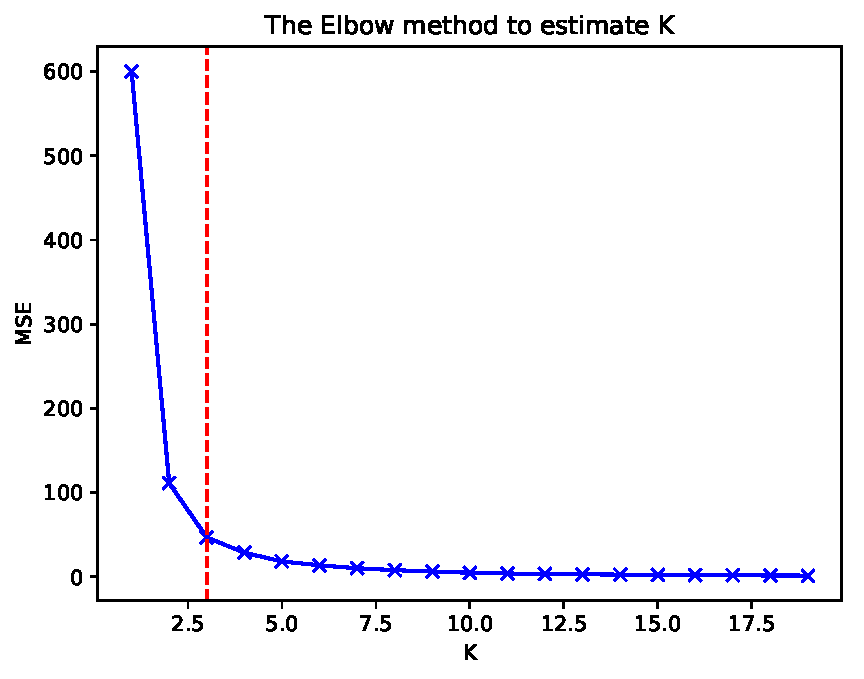
\includegraphics[width=0.5\linewidth]{Iris_elbow_determination_k.pdf}
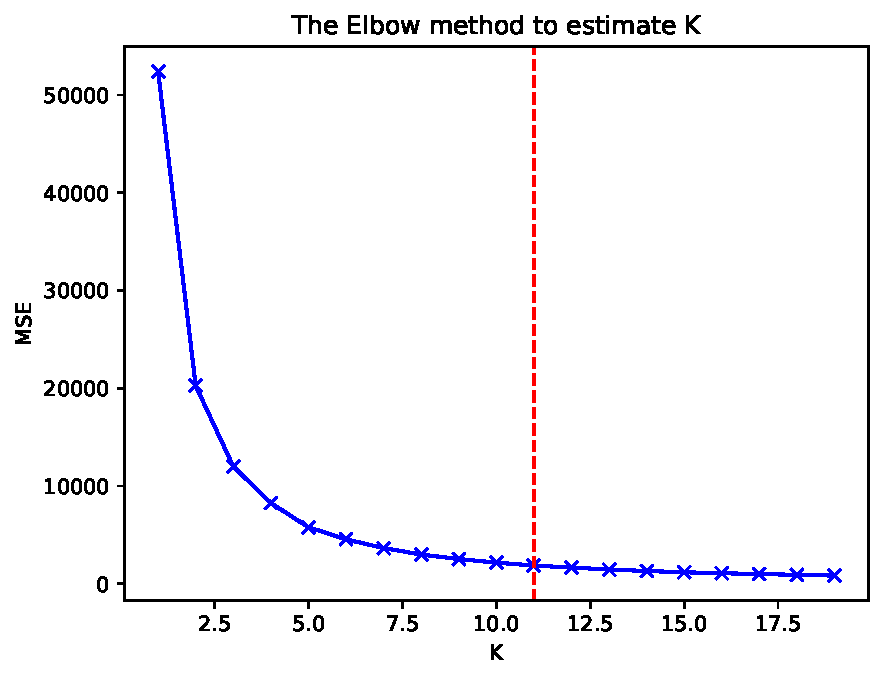
\includegraphics[width=0.5\linewidth]{Fault_Steel_Plates_elbow_determination_k.pdf}
\end{minipage}
\end{figure} 

\subsection*{The nearest neighbor method for estimating eps\_dbscan and min\_pts\_dbscan}

There were no major changes made for this method. I closely followed the steps mentioned in the notes, except that I choose the number of nearest neighbors $K$ to be 5 instead of $n$ - 1. This was done because the empirical evidence did not show any advantage of using a $K \geq 6$.

To choose the \texttt{eps\_dbscan} and \texttt{min\_pts\_dbscan}, I again computed a $cost_k$ for each neighbor $k \in K$, given as :

\begin{equation}
cost_k = argmin_{1 \leq j \leq n} dist[j] + 0.05 \cdot || J ||_2
\end{equation}

where $dist[j]$ was the distance $j$th entry of the $k$ th column in the k-dist graph and $|| J ||_2$ represents the l2 norm of $J$, that is, $range(0, j)$. The idea here again was to penalize more number of points ($j$). However, this time I had to lower down the penalty by 5\%, which seemed to work the best.

The smallest $cost_k$ was chosen to determine,  \texttt{eps\_dbscan} and \texttt{min\_pts\_dbscan}.

Figure~2 shows \texttt{eps\_dbscan} and \texttt{min\_pts\_dbscan} picked up for Iris and Faulty Steel Plates dataset.

\begin{figure}
\begin{minipage}{\linewidth}
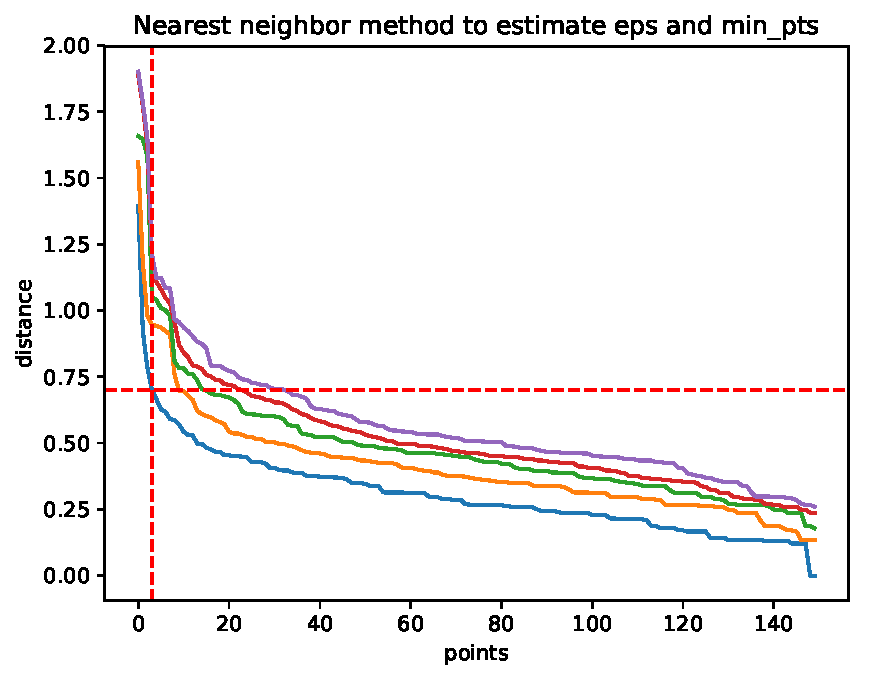
\includegraphics[width=0.5\linewidth]{Iris_nn_determination_minpts_eps.pdf}
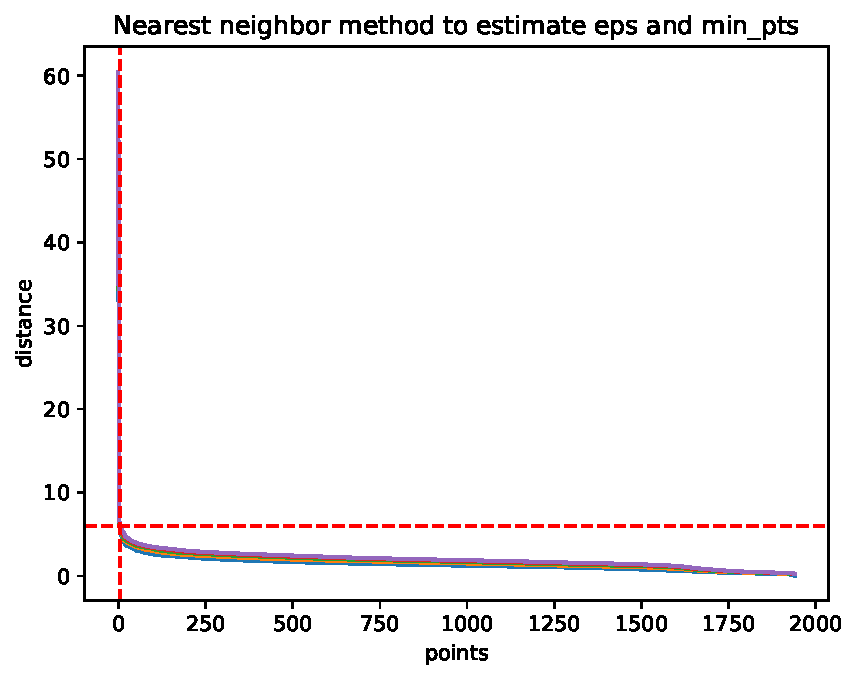
\includegraphics[width=0.5\linewidth]{Fault_Steel_Platesnn_determination_minpts_eps.pdf}
\end{minipage}
\end{figure} 

\section*{Performance evaluation}

I computed the runtime, SSE and chi-square to judge the quality of the clustering methods. The chi-square method is an interesting way to utilize the class labels $Y$ and see if the cluster labels were highly associative with $Y$. I used the p-value to determine the strength of association, a lower p-value better.

\subsection*{Performance on Iris Data-set}

\begin{table}[!hptb]
\centering
\begin{tabular}{|l|c|c|c|c|}
\hline
\textbf{Info} & \textbf{Kmeans} & \textbf{Agnes.scipy} & \textbf{Agnes.sklearn} & \textbf{DBSCAN} \\\hline
\textbf{runtime} & 0.029 & 0.003 & 0.0018 & 0.108 \\
\textbf{sse} & 139.8 & 148.8 & 148.8 &	225.2 \\
\textbf{chisq p-value} & 1.71E-39 & 5.03E-40 & 5.03E-40 & 9.95E-32 \\\hline
\end{tabular}
\caption{Result on `Iris' data-set with `standard' configuration of 4  clustering methods.}
\end{table}

Table~1 shows the runtime (in seconds), SSE and chisq-pvalue scores for `Iris' data-set using the `standard' configuration on 4 clustering algorithms : Kmeans, Agnes.scipy (Agglomerative clustering from scipy), Agnes.sklearn (Agglomerative clustering from sklearn) and DBSCAN. The data-set was scaled using the `StandardScaler' method from sklearn. DBSCAN performs the worst on this data-set, however, I think it is expected as this dataset has more blobs than continuous patterns. Interestingly, even though Kmeans has a lower SSE, the association between the cluster labels and ground truth $Y$ were better captured by the Agglomerative methods.

\subsection*{Performance on Faulty steel plates Data-set}

I merged the 7 class label columns into one class label as the `fault' always belonged to one class column for each sample.

\begin{table}[!hptb]
\centering
\begin{tabular}{|l|c|c|c|c|}
\hline
\textbf{Info} & \textbf{Kmeans} & \textbf{Agnes.scipy} & \textbf{Agnes.sklearn} & \textbf{DBSCAN} \\\hline
\textbf{runtime} & 0.22 & 0.17 & 0.14 & 0.32 \\
\textbf{sse} & 20427.7 & 21564.9 & 21564.9 &	51401.9 \\
\textbf{chisq p-value} & 1 & 1 & 1 & 1 \\\hline
\end{tabular}
\caption{Result on `Faulty Steel Plates' data-set with `standard' configuration of 4  clustering methods.}
\end{table}

Table~2 shows the runtime (in seconds), SSE and chisq-pvalue scores for `Faulty Steel Plates' data-set using the `standard' configuration on 4 clustering algorithms : Kmeans, Agnes.scipy (Agglomerative clustering from scipy), Agnes.sklearn (Agglomerative clustering from sklearn) and DBSCAN. The data-set was scaled using the `StandardScaler' method from sklearn. All methods do very poorly for this dataset (p-value is at its highest value of 1), however, DBSCAN was again the worst performer. Again, I think this dataset has more blobs than continuous patterns.

\section*{A more comprehensive evaluation}

Since most of the parameters were automatically computed, the only parameters I could have changed were \texttt{linkage\_method} and \texttt{dist\_metric}, however, there were no major changes except when I changed \texttt{dist\_metric} to `cosine', all performances dropped. However, this was expected as `cosine' distance does well for text clustering where the magnitude of the distance does not matter.

\end{document}